\subsection{Digital front end}\label{sec:frontend}
The digital front end (DFE) consist of three parts, D flip flop with a NAND and a NOR port. This can been seen in Fig. ~\ref{fig:Global_schematic_DFE_figure}. The D flip flop will synchronise the incoming data and the NAND/NOR gate will up-modulate the signal with the local oscillator in the digital domain. In comparison with the global schematic of the previous group (Appendix: Fig. ~\ref{fig:Global_schematic_previous_group_figure}) the DFE consist of one less D flip flop in the diagram. This will increase the synchronisation of nmos and pmos of the current sources. The DFE works in a high frequency domain and it needs to switch fast. Therefore thin oxide transistors are used. The drawback of this kind of transistors is that they operate at low voltages (max 1.2V), so less power at the output stage. To solve this problem a level shifter is used to increase the power at the output stage. The level shifter is described in paragraph ~\ref{sec:levelshifter}. 

\begin{figure}[h]
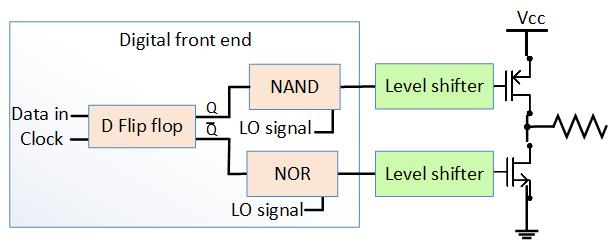
\includegraphics[width=0.5\textwidth]{Global_schematic_DFE.jpg}
\caption{One side of the diagram of the new digital front end.}
\label{fig:Global_schematic_DFE_figure}
\end{figure}

\subsubsection{D flip flop}\label{sec:frontend}
A D flip flop will be used to synchronise the incoming thermometer coded data to ensure that the transistors of the output stage switch at the same time. There are a couple of challenges that are important to take into account when designing a D flip flop, for example the operation speed and the transition time of the output at the rising clock.
A flip flop can be made in different ways. The two main technologies are in CMOS and CML. The CMOS design is relatively less complex in compare to CML, but in CML there are more parameters that can be modified to tune the output. In this project the CMOS design is used, because it is less complex, single-ended and it can be realised in a short time period. 

The CMOS circuit of the previous group is been used as basic circuit. ~\cite{powerdac} - ~\cite{coursebook}. The old schematic can been seen in the appendix Fig.~\ref{fig:D_flip_flop_ previous_group_figure}. The new schematic consist of 32 transistors and is showed in Fig.~\ref{fig:D_flip_flop_schematic_figure}. There are three changes made in compare with the old schematic. The first change is that a second output is been added to flip flop, as mentioned before to reduce one flip flop in the total schematic. The second change is a nmos switch is added to improve the synchronisation between the output and the input. The last change is that the sizes of the nmos and the pmos transistors are changed, to reduce the delay of the output. The size of the nmos and pmos will be further discussed, first the basic principle of a D flip flop is explained. 

\begin{figure}[h]
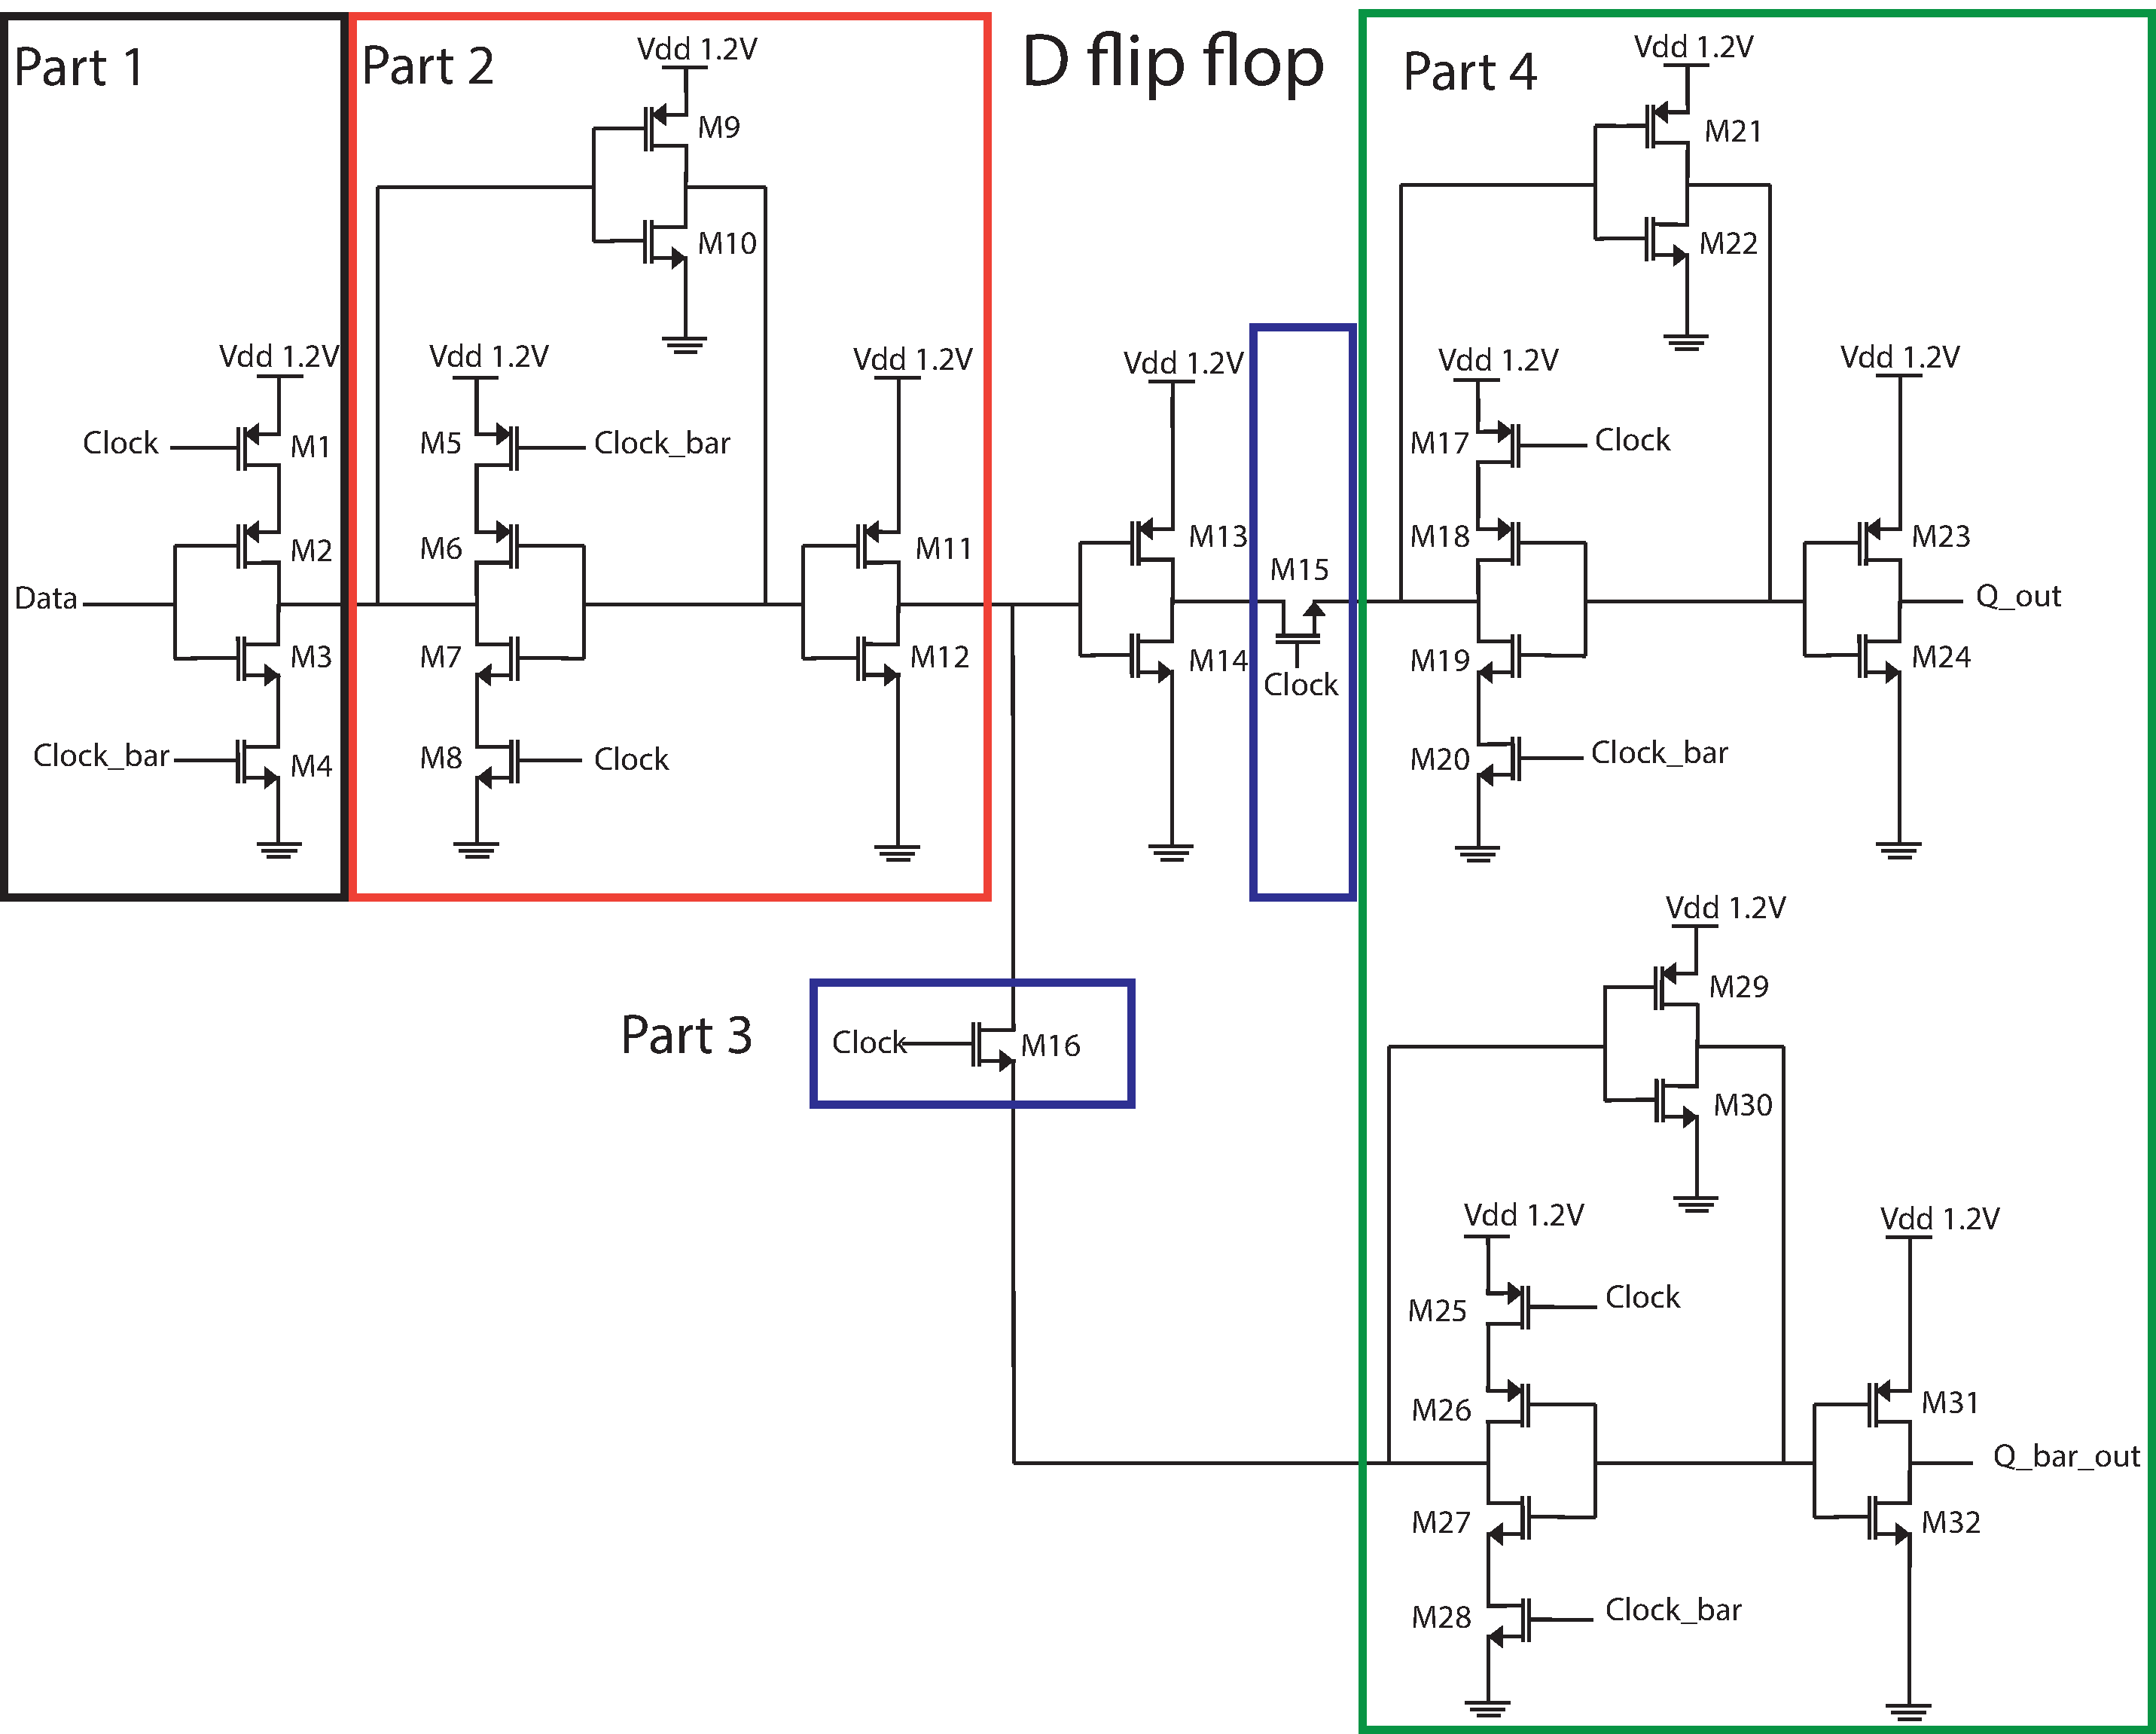
\includegraphics[width=0.5\textwidth]{D_flip_flop_new_schematic.pdf}
\caption{The improved D flip flop schematic.}
\label{fig:D_flip_flop_schematic_figure}
\end{figure}

To explain the principle of a master-slave D flip flop, the schematic can be divided into four parts, settle time of the data, master latch, two switches and slave latch. In the first part the data will be set when the clock is low. The second part, the master will follow the signal of the first part when the clock is low and hold the data when the clock is high. In the third part the switches will be closed when the clock is high. The slave latch(part 4) can set the data and when the clock is high it will hold the data.
The size of the pmos and nmos of part one, two and four are the same. The size of the nmos is set on 50nmx90nm (length x width). The length of the pmos is the same, but the width of the pmos is determined with a parameter sweep to get the smallest delay of transition. In the parameter sweep the clock frequency is set on 1 GHz and the data frequency is set on 500MHz. The results are showed in the appendix in Fig.~\ref{fig:parametersweep_changing_w_high_to_low_figure} and Fig.~\ref{fig:parametersweep_changing_w_low_to_high_figure}. The optimal width of the pmos is 120nm. It has the smallest delay of transition.  The ratio of the width of the pmos and nmos will be 1.33:1.

The size of the switching nmos (part 3) is also determined with a parameter sweep with the same setting. The results are shown in Fig.~\ref{fig:Parameter_sweep_changing_w_of_the_swiching_nmos_high_to_low_figure} and Fig.~\ref{fig:Parameter_sweep_changing_w_of_the_swiching_nmos_low_to_high_figure} in the appendix. The optimal value of the width is 280nm. The results of this value is compared with the previous schematic and is shown in Fig.~\ref{fig:Comparison_old_schematic_and_new_schematic_low_figure} and Fig.~\ref{fig:Comparison_old_schematic_and_new_schematic_high_figure}. The overall delay of transition is reduced with 12ps to 13ps of Q and Q bar, but only transition from low to high of Q bar is slightly increased with 2 ps. 

\begin{figure}[h]
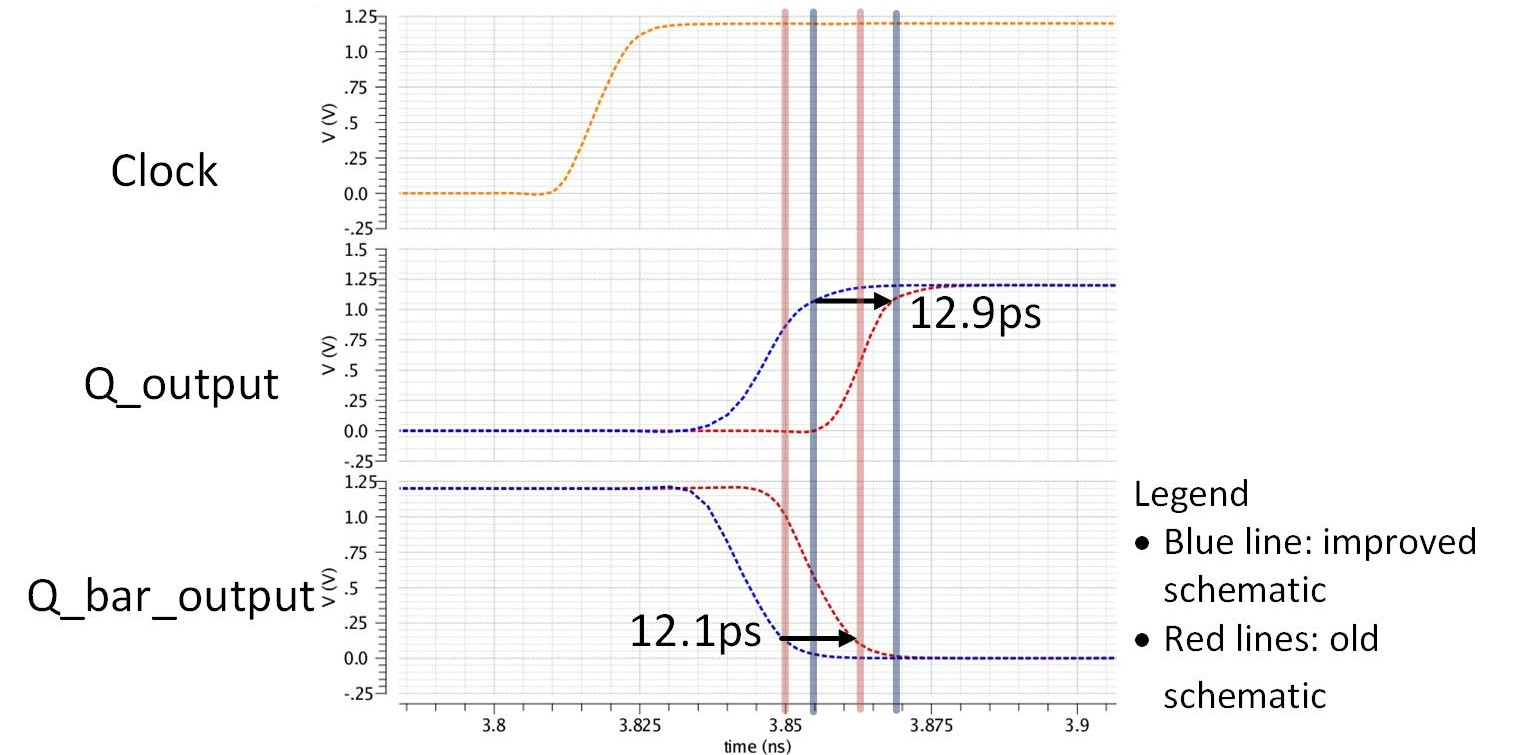
\includegraphics[width=0.5\textwidth]{Comparison_old_schematic_and_new_schematic_high.jpg}
\caption{Comparison of the delay of transition between the old schematic and the new schematic when the data is high }
\label{fig:Comparison_old_schematic_and_new_schematic_high_figure}
\end{figure}

\begin{figure}[h]
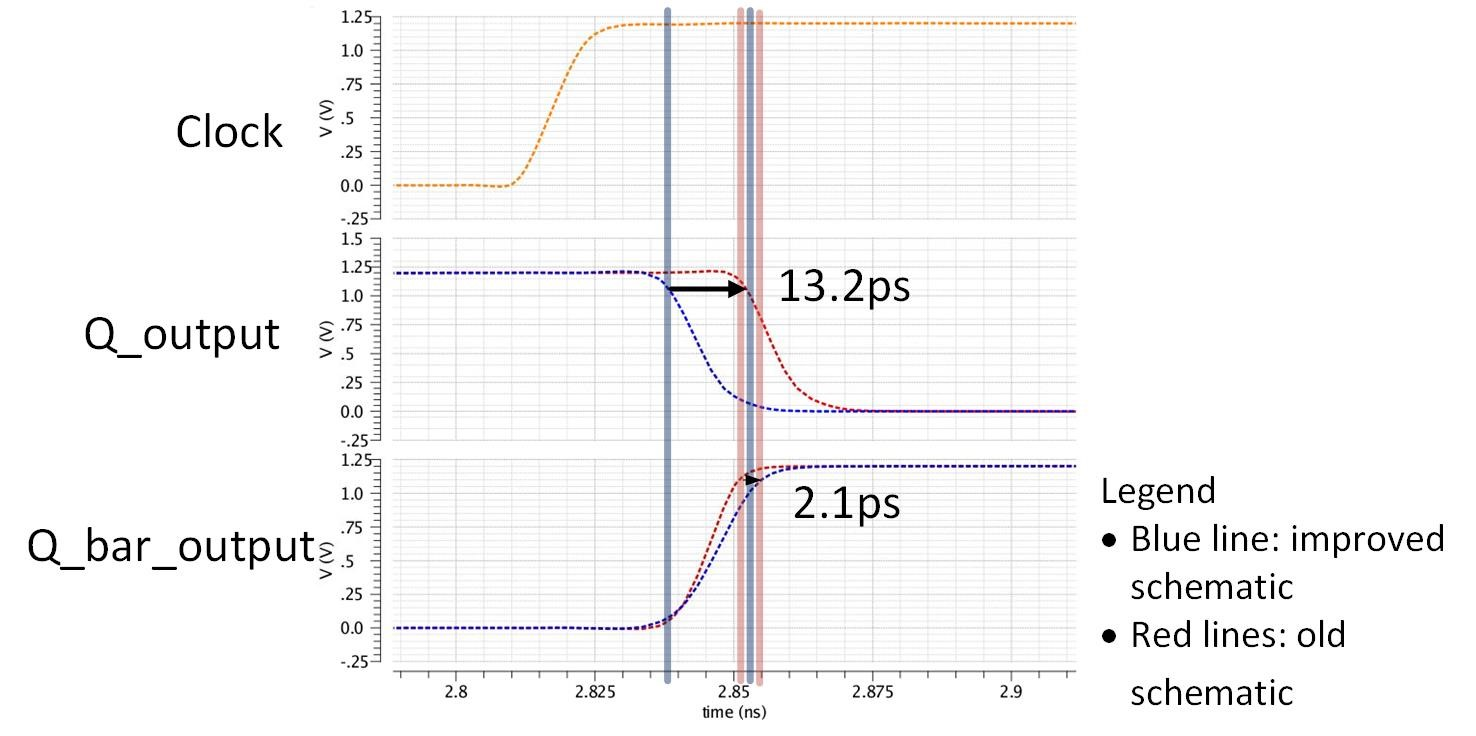
\includegraphics[width=0.5\textwidth]{Comparison_old_schematic_and_new_schematic_low.jpg}
\caption{Comparison of the delay of transition between the old schematic and the new schematic when the data is low.}
\label{fig:Comparison_old_schematic_and_new_schematic_low_figure}
\end{figure}

With all the transistors sizes known the critical point can be measured. The minimal time that the data needs to be set is 40ps before the clock is high. The transition delay of Q and Q bar is 29ps when the data is high. When the data is low the delay of Q is 27ps and Q bar is 32ps. This is shown in Fig.~\ref{fig:Critical_values_data_high_to_low_figure} and Fig. ~\ref{fig:Critical_values_data_low_to_high_figure}.

In conclusion, in the new schematic the delay of the transition has been reduced and this improves the synchronisation of circuit.   

\begin{figure}[h]
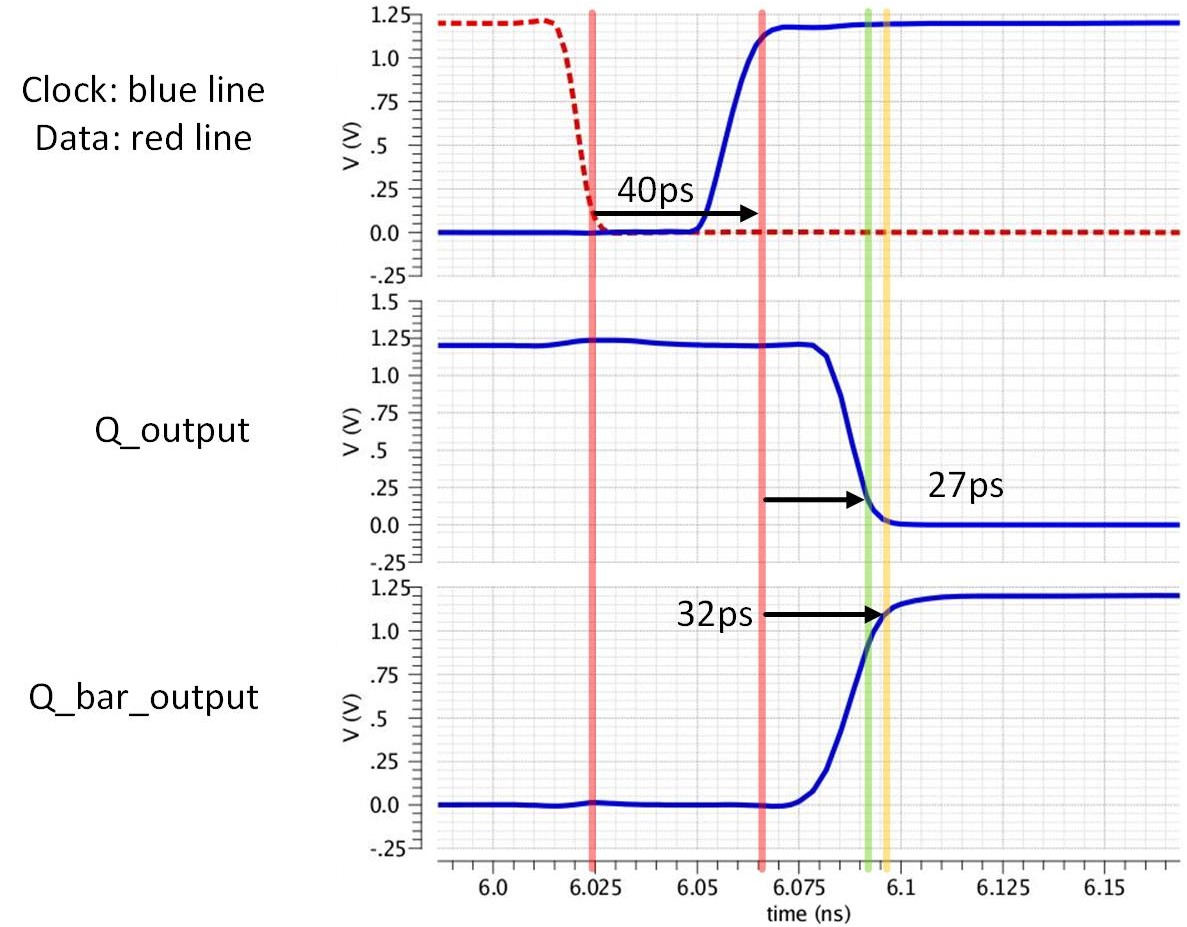
\includegraphics[width=0.5\textwidth]{Critical_values_data_high_to_low.jpg}
\caption{The critical values when the data goes from high to low}
\label{fig:Critical_values_data_high_to_low_figure}
\end{figure}

\begin{figure}[h]
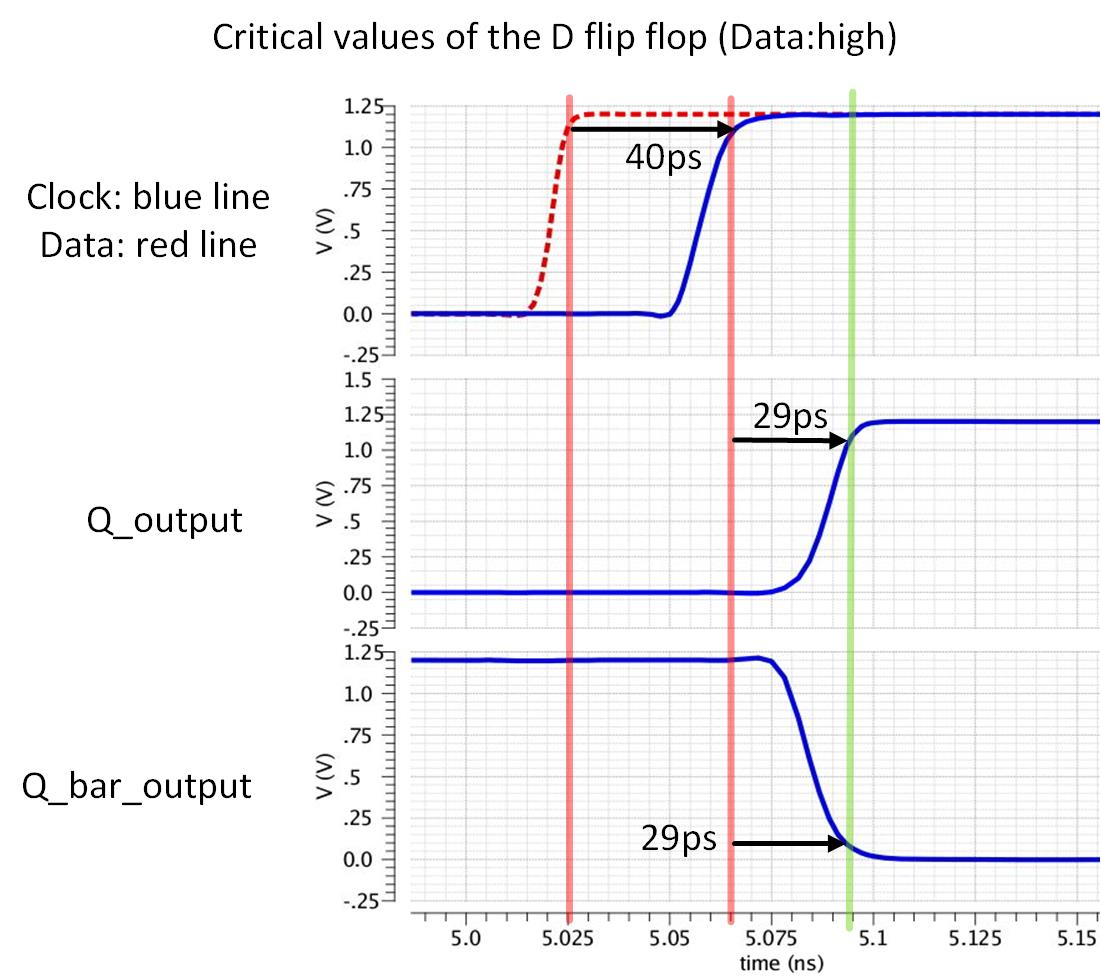
\includegraphics[width=0.5\textwidth]{Critical_values_data_low_to_high.jpg}
\caption{The critical values when the data goes from low to high.}
\label{fig:Critical_values_data_low_to_high_figure}
\end{figure}

\subsubsection{NAND/NOR gate}\label{sec:frontend}
The NAND and NOR will up-modulate the local oscillator signal (LO) with the data from the D flip flop. This will happen in the digital domain with an LO signal of 2Ghz square wave.
The design of a NAND and NOR is shown in Fig.~\ref{fig:NAND_schematic_figure} and Fig.~\ref{fig:NOR_schematic_figure}.

\begin{figure}[htp]
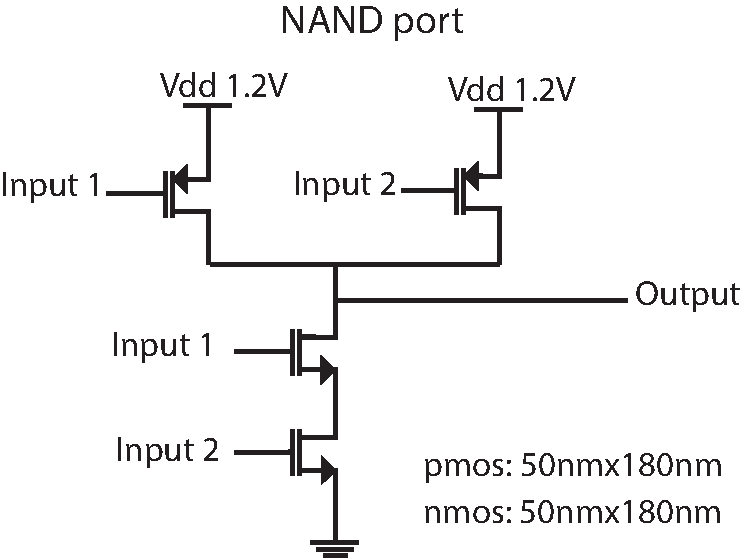
\includegraphics[width=0.4\textwidth]{NAND_schematic.pdf}
\caption{The schematic of the NAND port.}
\label{fig:NAND_schematic_figure}
\end{figure}

The NAND port has two pmos in parallel and 2 nmos in series. In a normal cmos inverter the width of the pmos is 2 times larger than the nmos. The size of the pmos is 50nmx180nm (length x width).  In this situation two nmos transistors are in series. The size of the nmos is been determined with a parameter sweep. The result is shown in the appendix in Fig.~\ref{fig:NAND_nmos_sweep_figure}. The optimal value 180nm is chosen, because it has the same fall and rise time. The size of the nmos and pmos is 50nmx180nm (length x width).

\begin{figure}[htp]
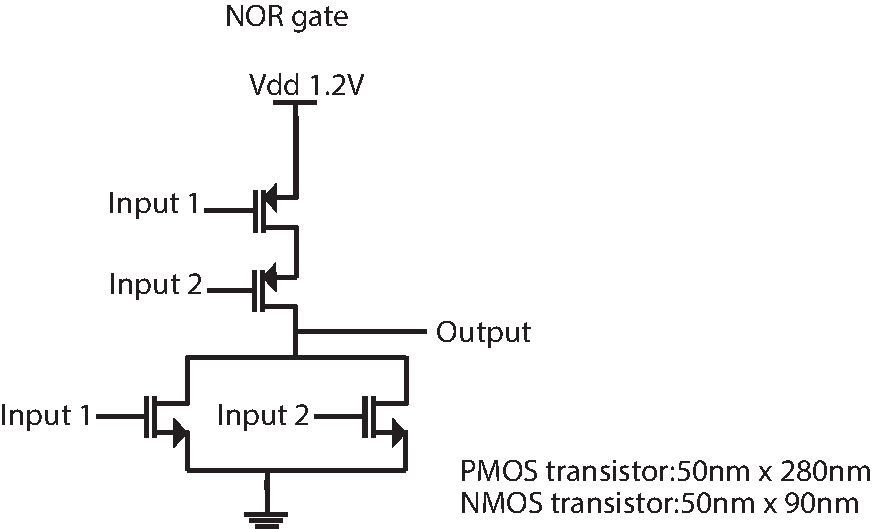
\includegraphics[width=0.35\textwidth]{NOR_schematic.pdf}
\caption{The schematic of the NAND port.}
\label{fig:NOR_schematic_figure}
\end{figure}

The NOR port has two pmos in serie and 2 nmos in parallel. The size of the nmos will be the smallest value: 50nmx90nm (length x width). The width of the pmos will be determined with a parameter sweep. The result is shown in the appendix in Fig.~\ref{fig:NOR_pmos_sweep_figure}. The optimal value 280nm is chosen, because it has the same fall and rise time. The size of the pmos is 50nmx280nm (length x width).
